\chapter{TINJAUAN PUSTAKA}
% contoh opsi lain Bab 2
%\chapter{DASAR TEORI}


\section{Landasan Teori}
\noindent Penelitian ini didasarkan pada beberapa landasan teori yang relevan dengan segmentasi mikrovaskular ginjal menggunakan Fully Convolutional Network (FCN). Landasan teori ini meliputi pemahaman mendalam tentang mikrovaskular ginjal, konsep whole slide image (WSI), prinsip-prinsip deep learning, dan arsitektur FCN.

\subsection{Mikrovaskular Secara Umum}


\noindent Mikrovaskular, sebagai cabang terkecil dari pembuluh darah, memainkan peran penting dalam berbagai fungsi tubuh manusia. Struktur ini, dengan ukuran kurang dari 100 mikrometer, terdiri dari arteriol, kapiler, dan venula \cite{mescher_junqueiras_2021,pepe_microvascular_2023}. Arteriol merupakan pembuluh darah kecil (diameter 10-100 $\mu$m) dengan ujung yang pada dindingnya terdapat otot halus berperan sebagai sfingter untuk mengatur aliran darah secara berkala ke dalam kapiler dan struktur ini juga bertindak sebagai pengatur tekanan darah. Kapiler merupakan pembuluh darah paling kecil (diameter 4-10 $\mu$m) dalam struktur mikrovaskular yang berfungsi sebagai tempat pertukaran metabolit antara darah dan jaringan \cite{haffner_emerging_2023}. Oksigen dan nutrisi berdifusi dari darah ke jaringan, sementara karbon dioksida dan produk sisa diangkut dari jaringan ke darah. Venula merupakan pembuluh darah kecil (diameter 10-100 $\mu$m) tempat berlanjutnya aliran darah dari kapiler dan membawanya ke vena. Struktur ini juga berperan sebagai tempat keluarnya leukosit (sel darah putih) untuk mengatasi infeksi atau peradangan pada jaringan.

\noindent Secara umum mikrovaskular memiliki peran penting dalam sirkulasi darah dan pertukaran zat diseluruh tubuh \cite{rusanova_role_2022}. Struktur ini membantu setiap sel tubuh manusia menerima oksigen dan nutrisi agar bisa berfunsi secara optimal. Selain itu, struktur ini juga berfungsi sebagai alat untuk membuang sisa metabolisme sehingga tubuh tidak akan keracunan akumulasi zat sisa metabolisme.

\noindent Studi tentang mikrovaskular sangat penting dalam bidang kesehatan dan patologi. penelitian internasional yang sedang berlangsung oleh Chan Zuckerberg Initiative's Human Cell Atlas (HCA), Knut and Allice Wallenberg Foundation's Human Protein Atlas (HPA) dan National Institutes of Health's Human BioMolecular Atlas Program (HuBMAP) yang bernama Common Coordinate Framework (CCF) memanfaatkan mikrovaskular sebagai sistem koordinat dalam tubuh manusia untuk memetakan setiap sel di seluruh tubuh manusia \cite{weber_considerations_2020}. penelitian tersebut dilakukan untuk memahami spesialisasi, interaksi dan organisasi spasial setiap sel dalam tubuh manusia.

\noindent Pemanfaatan mikrovaskular sebagai kordinat pada projek CCF tersebut bisa dilakukan karena pembuluh darah  mengikuti setiap jalur unik di setiap organ sehingga bisa mencermnkan sifat biologis khusus setiap jaringan \cite{weber_considerations_2020}. Kerumitan struktur mikrovaskular mencerminkan kompleksitas organ dan jaringan yang dilaluinya, sehingga dapat menyoroti ketergantungan antara mikrovaskular dan sel dalam menjalankan fungsi yang tepat. 



\subsection{Ginjal dan Mikrovaskular Ginjal}


\noindent Ginjal adalah organ vital yang bertanggung jawab untuk menyaring darah, mengatur tekanan darah, dan menjaga keseimbangan elektrolit dalam tubuh manusia \cite{sultan_microvasculature_2023,ito_s-27-1_2023,bagarao_renal_2023}. %+\citeabdulla_biology_2022
 Ginjal melakukan hal tersebut melalui proses-proses seperti filtrasi glomelurus, penyerapan tubulus, dan sekresi tubulus, yang pada akhirnya membentuk urin \cite{auctores_publishing_llc_what_2021}. Selain itu ginjal memainkan peran penting dalam memproduksi hormon seperti eritropioietin, yang meransang produksi darah merah dan renin, yang terlibat dalam pengaturan tekanan darah \cite{scannali_s-22-6_2023}. Kemudian, ginjal membantu mengatur volume cairan tubuh, kandungan elekrolit, dan keasaman, serta membuang produk limbah dan racun dalam tubuh. Secara garis besar, ginjal sangat penting untuk menjaga lingkungan internal tubuh, guna menjamin kondisi yang optimal agar berbagai proses tubuh dapat berfungsi dengan baik.
 

\noindent Fungsi-fungsi vital ginjal dilakukan oleh struktur-struktur khusus di dalamnya, terutama pada bagian korteks, medula, dan papila. Masing-masing bagian ini memiliki peran unik dalam proses filtrasi, reabsorpsi dan sekresi yang terjadi di ginjal. korteks merupakan area terluar ginjal yang memiliki sel-sel bulat ginjal yang membungkus glomelurus sebagai alat untuk menyaring darah \cite{gopalan_renal_2022}. Area juga memiliki nefron proximal convoluted tubules (PCT) dan distal convoluted tubules (DTC) yang berperan untuk reabsorsi dan sekresi \cite{mescher_junqueiras_2021}. Diantara struktur tubular tersebut terdapat jaringan kapiler kompleks yang disebut kapiler peritubular.  Medula merupakan area dalam dalam ginjal terdiri dari tubulus-tubulus nefron (lengkung Henle dan duktus kolektivus) dan pembuluh struktur kapiler khusus medula bernama vasa recta yang berperan dalam pengatur konsentrasi urin \cite{haug_multi-omic_2022}. Dalam pengaturan konsentrasi urin medula ginjal, terjadi mekanisme countercurrent multiplication di lengkung Henle dan mekanisme countercurrent exchange di vasa recta \cite{nankivell_importance_2020}. Gradien osmotik yang terjadi akibat mekanisme-mekanisme tersebut memungkinkan ginjal untuk menyaring kembali air dari filtrat glomelurus, sehingga menghasilkan urin yang lebih pekat. Papila merupakan sub bagian dari medula yang merupakan dasar dari piramida ginjal berfungsi sebagai tempat pengumpulan urin sebelum di teruskan ke kaliks minor \cite{sabate_arroyo_relationship_2020}

\noindent Mikrovaskular ginjal memiliki beberapa komponen unik yang berperan penting dalam proses pembentukan urin dan pengaturan fungsi ginjal, mencakup glomelurus, kapiler peritubular, vasa recta, arteriol aferen dan arteriol eferen \cite{mescher_junqueiras_2021}. Glomelurus merupakan kumpulan kapiler yang terdapat di kapsul Bowman yang berfungsi sebagai alat penyaring darah sehingga air dan limbah bisa melewati dinding kapiler ke dalam kapsul Bowman, sementara sel darah dan protein besar tetap berada di dalam aliran darah \cite{luxen_unique_2023}. kapiler peritubular merupakan kapiler yang mengelilingi tubulus ginjal yang berperan mereabsorsi cairan penting yang tidak tersaring di dalam glomelurus \cite{savedchuk_targeting_2023}. Vasa recta merupakan kapiler yang terletak di medula ginjal, mengelilingi  lengkung henle yang berfungsi menjaga gradien osmotik untuk proses reabsorsi air dari duktus kolektivus \cite{goligorsky_emerging_2022}. Arteriol aferen dan eferen merupakan arteriol  yang berfungsi dalam transportasi darah dari dan ke glomlurus \cite{ergin_kidney_2021}.


\subsection{Whole Slides Image (WSI)}

\noindent Whole Slide Image (WSI) merupakan teknologi dalam pengambilan gambar histologi yang melibatkan pemindaian slide mikroskopik menjadi gambar digital beresolusi tinggi \cite{hanna_whole_2020}. Gambar yang dihasilkan dari pemindaian WSI biasanya berukuran besar (ratusan hingga ribuan megabyte) yang di simpan dalam berbagai format, termasuk SVS, SCN, MRXS, NDPI, TIFF, dan DICOM. Penggunaan WSI dalam pemindaian slide mikroskopik ini dapat meningkatkan reproduksibilitas analisis dan mengurangi kesalahan manusia dalam interpretasi visual \cite{li_hardware-software_2023}. Dalam dunia patologi WSI juga dimanfaatkan untuk berbagai keperluan termasuk: diagnosis primer dimana dalam pembuatan diagnosis tanpa melihat ke dalam slide kaca secara langsung, konsultasi jarak jauh dengan berbagai WSI secara digital dan penelitian yang melibatkan analisis WSI untuk penelitian biomolekular, penemuan obat baru dan pengembangan alat diagnostik.


 
\subsection{Segmentasi Gambar}

\noindent Segementasi gambar merupakan sebuah tugas penting dalam anilisis gambar histologis dan medis. Proses ini akan mempartisi gambar digital menjadi wilayah yang terpisah (tidak tumpang tindih), yang masing-masing wilayah  berhubungan dengan suatu objek atau struktur yang relevan dalam lingkup pengamatan \cite{wu_image_2023}. Dengan kata lain, segmentasi gambar merupakan proses mengelompokkan piksel-piksel dalam gambar berdasarkan karakteristik tertentu. Hasil dari segmentasi gambar adalah sekumpulan segmen yang mewakili objek dari objek yang berbeda dalam gambar. Metode yang di gunakan dalam proses ini sangat bervariasi, dari yang metode sederhana seperti: treshholding memisahkan piksel berdasarkan intensitasnya, region growing mengelompokkan piksel-piksel berdasarkan kemiripan, clustering memisahkan piksel berdasarkan kemiripan dalam fitur multidimensi dan aktive countour menggunakan kurva yang dapat berubah untuk mendeteksi objek, hingga metode deep learning seperti FCN yang lebih canggih \cite{huang_fully_2022,wang_comprehensive_2022}

\noindent Dalam praktiknya segmentasi gambar menggunakan deep learning terbagi ke dalam dua jenis: segmentasi semantik dan segmentasi instance. Segmentasi semantik merupakan jenis segmentasi untuk mencari pemahan rinci terhadap berbagai wilayah dalam gambar yang mana pada jenis ini pelabelan setiap piksel dalam gambar didasarkan setiap kelas objek \cite{fan_image_2023}. Di sisi lain, segmentasi instace melabeli piksel objek dalam gambar tidak hanya didasarkan setiap kelas dari objek tetapi, juga membedakan antara instance objek  secara individu walaupun ada dalam kelas yang sama sehingga memungkinkan untuk penggambaran yang tepat dari setiap objek yang ada dalam gambar. Kedua jenis segmentasi ini telah dimanfaatkan dalam berbagai bidang seperti analisis gambar lalulintas untuk sistem kemudi otomatis, transfer gaya gambar dalam komputer vision dan analisis struktur mikrovaskular sebagaimana yang akan dilakukan pada penelitian ini \cite{wang_traffic_2023, zhang_image_2023, sultan_microvasculature_2023}


\subsection{Deep Learning}

\noindent Deep learning merupakan sub bidang dari machine learning yang menggunakan jaringan syaraf tiruan dengan banyak layer untuk mempelajari pola dari suatu data \cite{goodfellow_deep_2016,yang_deep_2023}. Perkembangan deep learning memberikan pengaruh besar pada analisis citra medis \cite{sistaninejhad_review_2023}. Dimana pada tahap awal perkembangan analisa citra medis, fitur-fitur diektraksi secara tradisional menggunakan teknik pemrosesan citra tradisional yang memakan waktu dan butuh validasi ahli \cite{huang_fully_2022}.  Kemudian, dengan munculnya deep leaning terutama Convolutional Neural Network (CNN), proses ektraksi fiturpun menjadi otomatis \cite{huang_fully_2022,azad_medical_2022}. 

\noindent CNN merupakan jenis arsitektur jaringan saraf tiruan yang sangat efektif untuk tugas-tugas pengolahan citra, seperti klasifikasi gambar dan segmentasi gambar \cite{celeghin_convolutional_2023}. CNN bekerja dengan cara mengekstraksi fitur-fitur penting dari gambar melalui serangkaian lapisan konvolusi, pooling, dan aktivasi, yang memungkinkan model untuk mengenali pola dan struktur dalam data visual. Namun CNN tradisional memiliki keterbatasan untuk tugas segmentasi  gambar \cite{huang_fully_2022, azad_medical_2022, jasim_towards_2023}. Salah satunya berkaitan dengan fitur yang di ekstraksi model tersebut. Ketikan menggunakan kernel yang lebih kecil, fitur yang di hasilkan akan lebih lokal terhadap gambar asli, sehingga informasi global seperti lokasi mungkin hilang. Namun, ketika menggunakan kernel yang lebih besar, konteks dari fitur tersebut dapat berkurang.


\subsection{Fully Convolutional Network (FCN)}

Salah satu model deep learning yang sering digunakan dalam merupakan Fully Convolutional Network (FCN). Perbedaan antara FCN dan CNN tradisional terletak di layer terakhir bukan fully connected layer yang memungkinkan model untuk mengintegrasikan informasi . Namun, FCN mengganti layer terakhir sebagai output canel dengan jaringan konvolusi \cite{shlezinger_model-based_2023,huang_fully_2022}. Salah satu manfaat utama dari pendekatan ini adalah bahwa model tidak akan mendapatkan pembatasan dari fully connected layer, sehingga ukuran dari input akan lebih fleksibel \cite{iqbal_analyses_2023}.


Struktur FCN seperti pada gambar \ref{fig:fcn} menerapkan beberapa blok konvolusi yang terdiri dari lapisan konvolusi, aktivasi dan pooling pada jalur encoder untuk menangkap representasi semantik dari gambar \cite{azad_medical_2022}. Begitu juga, dalam jalur decoding FCN menggunakan lapisan konvolusi bersamaan dengan operasi upsampling untuk memberikan prediksi pada tingkat piksel sehingga model bisa melakukan tugas segmentasi \cite{deng_fcn_2023}. Skip conection juga digunakan dalam FCN untuk menemukan lokasi dari fitur di keseluruhan citra. 

\begin{figure}[H]
	\centering
	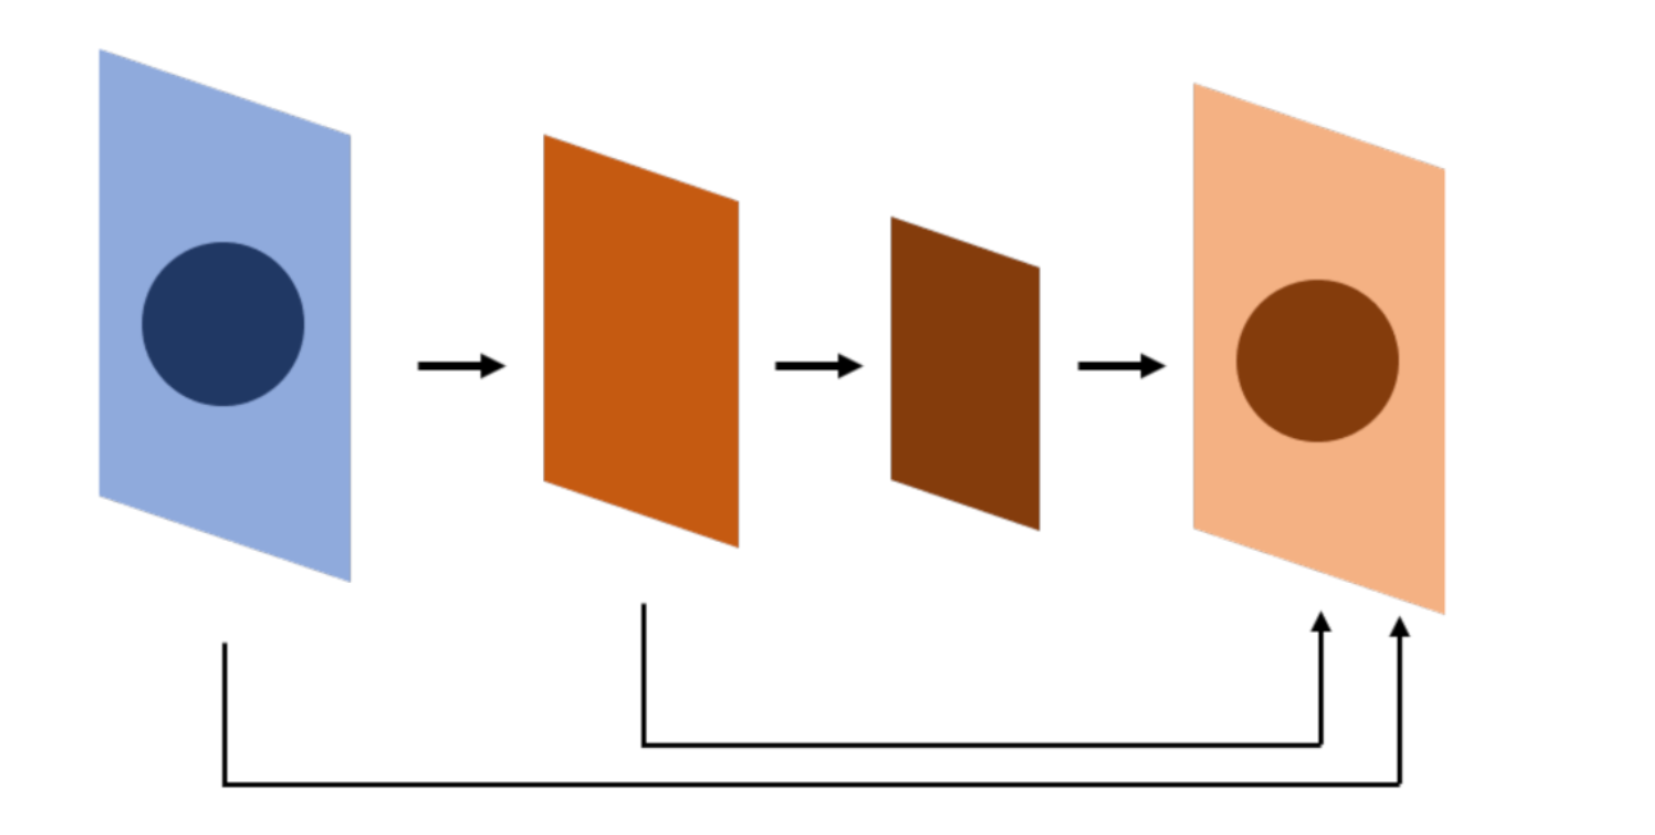
\includegraphics[scale=.2]{gambar/gambar-fcn.png}
	\caption{Jaringan FCN yang bagian terakhirnya di gantikan dengan blok konvolusi. FCN juga menggunakan skip connection untuk mentapkan lokasi dari fitur yang telah di ekstrak oleh encoder}
	\label{fig:fcn}
\end{figure}



\section{Menulis Persamaan}
\noindent Persamaan matematis dapat ditulis dalam berbagai bentuk. Beberapa faktor yang mempengaruhi penulisan antara lain: (1) apakah persamaan tadi perlu diberi nomor atau tidak (2) apakah ada persamaan-persamaan tadi dalam sebuah kelompok (3) atau apakah merupakan bentuk penurunan yang perlu disejajarkan (4) selain itu bisa juga persamaan yang ditulis di dalam teks.
\begin{equation}
E=mc^2
\end{equation}
    dengan $E$ adalah energi, $m$ adalah massa, dan $c$ adalah kecepatan cahaya.

\begin{equation}
\sqrt{x^2+1}
\end{equation}
    dengan $x$ adalah variabel.

